\begin{frame}[c]
\frametitle{A Theory of Onset Temperature in 2D: Spatial Correlations} %$J_\sigma$

\begin{columns}[T]

\begin{column}[T]{0.45\linewidth}

\begin{figure}[t]
\begin{overprint}
    \onslide<5->\centering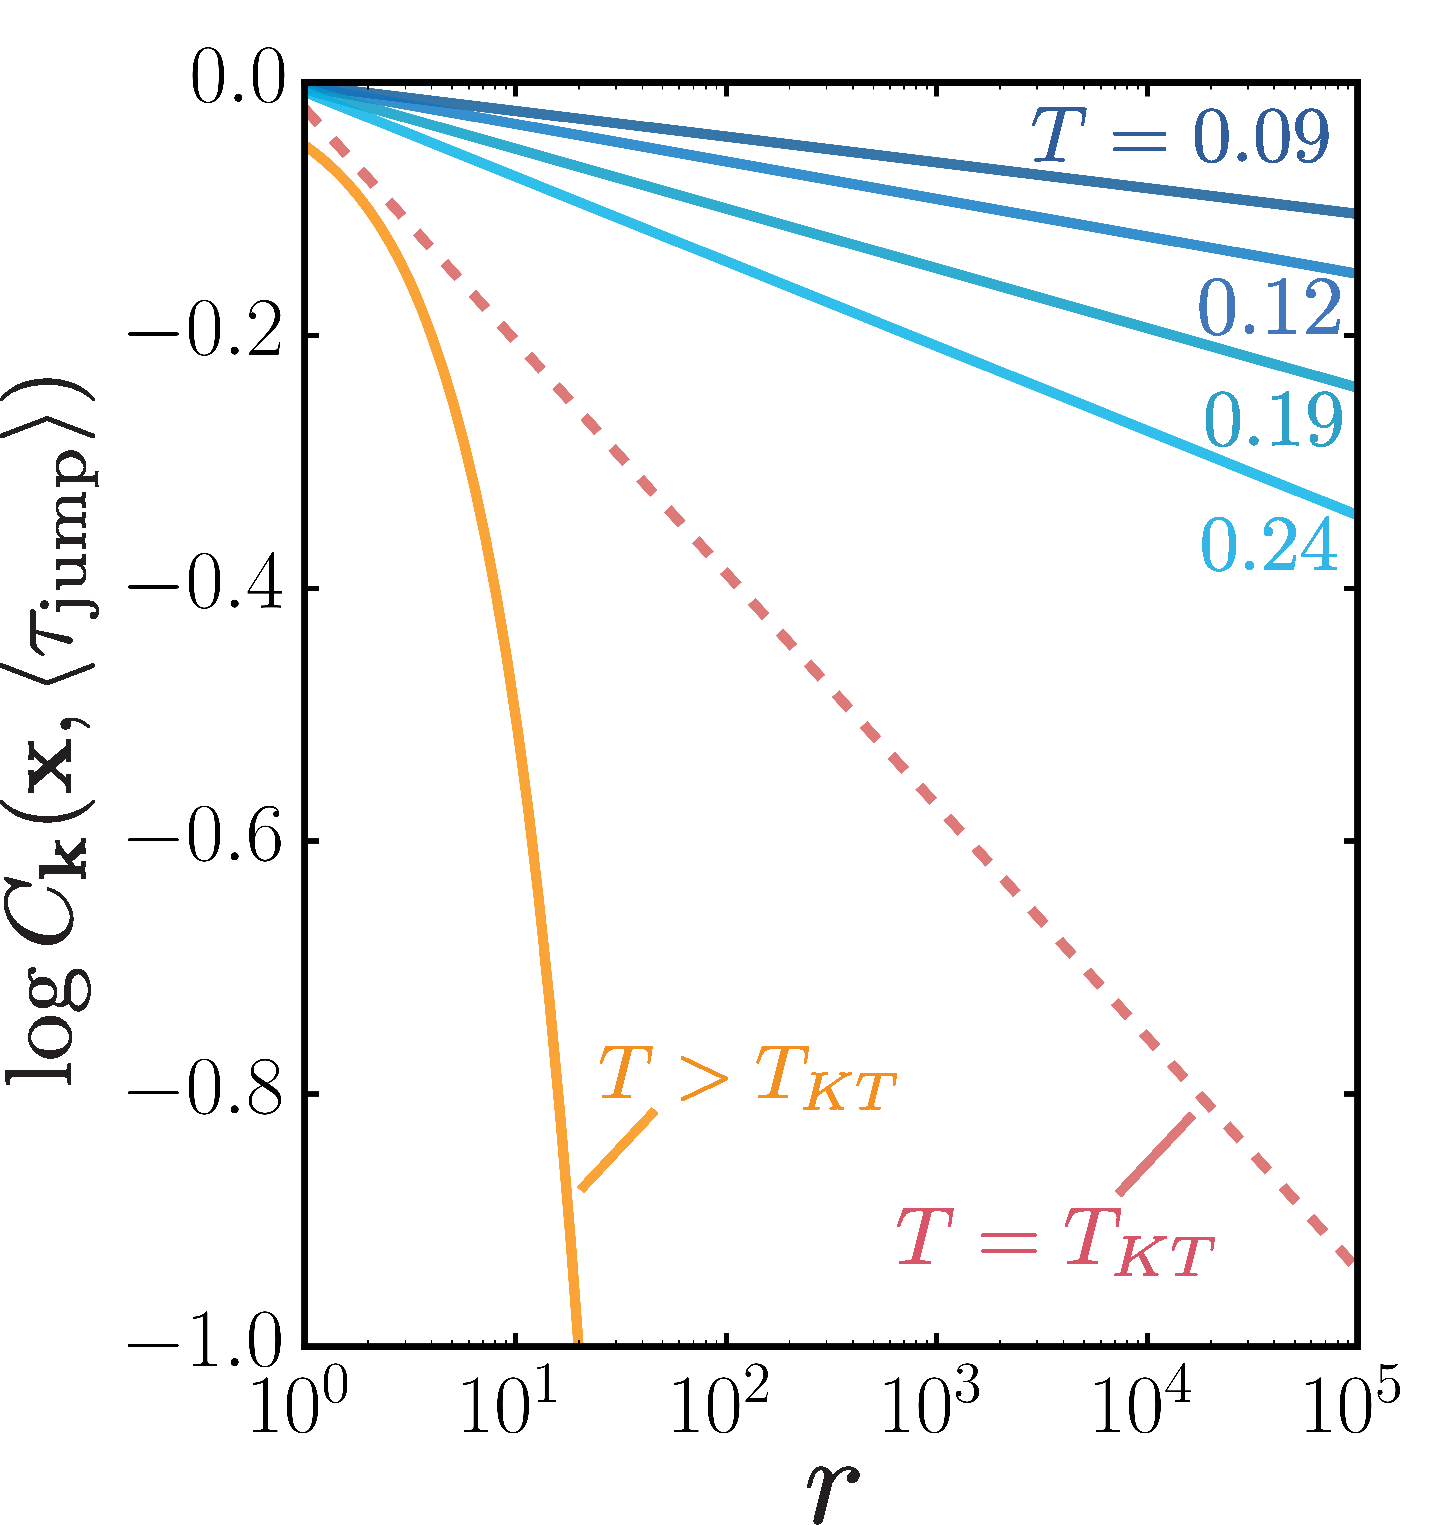
\includegraphics[height=0.75\textheight]{c.15-kt_spatialcorrel/spatialcorrel.pdf}\caption{Predicted spatial correlations for Poly-(12,0) $\varepsilon=0.2$. High-$T$ correlations decay exponentially.}
    %\onslide<5>\centering\includegraphics[height=0.675\textheight]{2.d-kt_thermoframework/Energy_Landcape_Voronoi.png}\caption{Testing a sentence that I want to write which will be this long}
\end{overprint}
\end{figure}

\end{column}

\begin{column}{0.55\linewidth}

\begin{itemize}
    \item<1-> The only major unverified prediction left is on \textit{spatial correlations}. \onslide<2->{Let $\rho_{\* k}( \* x,t) = e^{i \*k \cdot \* u(\* x, t)}$ be an order parameter.}
    \item<3-> Our theory predicts power-law decay:
    \onslide<4->{
    \begin{center}
    \begin{minipage}{0.85\textwidth}
    \begin{block}{\centering Low-$T$ Spatial Correlations}
    \vspace{-1em}
    \begin{align*}
    C_{\mathbf{k}}\left(\mathbf{x},\left\langle\tau_{\text {jump }}\right\rangle\right) &:= \left\langle\rho_{\mathbf{k}}\left(\mathbf{x},\left\langle\tau_{\text {jump }}\right\rangle\right) \rho_{-\mathbf{k}}(\mathbf{0}, 0)\right\rangle \\
     &\simeq\left(\frac{|\mathbf{x}|}{R}\right)^{-\sigma(k, T)}
     \\
    \sigma(k, T) &= k_{\mathrm{B}} T \frac{k^{2}\left(3-\nu^{\mathrm{R}}\right)\left(1+\nu^{\mathrm{R}}\right)}{4 \pi Y^{\mathrm{R}}}
    \end{align*}
    \end{block}
    \end{minipage}
    \end{center}
    }
    \item<6-> Testable by measuring displacement fluctuations at intermediate timescales but requires enormous system sizes to resolve (\textbf{future work})
\end{itemize}

\end{column}

\end{columns}

\end{frame}